\chapter{Wi-Fi Direct Middleware}
\label{chap2}
\thispagestyle{empty}

\noindent In this chapter, I'll show the low-level architecture of the \textsf{sPFWFDMid} module. In SPF2, I completely changed most of the code in this module. For this reason, you should consider completely deprecated this module from SPF1 and the related documentation.

\section{A quick overview}

All Wi-Fi Direct Middleware's code is into the \textsf{sPFWFDMid} sub-module. There are two main packages:

\begin{itemize}
	\item \textsf{wfd}: contains the entire logic.
	\item \textsf{wfdadapter}: contains all the classes and interfaces directly related to SPF.
\end{itemize}

When you open SPF on your smartphone, the first thing that happens, also before the start of the MainActivity, is the execution of the code into the \textsf{SPFApp.java}, that extends \textsf{Application}. 
The first thing that \textsf{SPFApp} does is inside its Application's class, where there is the initialization of SPF, with this line: \textsf{SPFContext.initialize(this, 0, true, WFDMiddlewareAdapter.FACTORY);}. As you can see, the only things that you must provide to this method are:
\begin{itemize}
	\item \textsf{context}: necessary to use all methods that require context into the Middleware.
	\item \textsf{goIntent} and \textsf{isAutonomous}: are values required by Wi-Fi Direct Middleware.
	\item \textsf{middleware}: to specify the middleware that you want to use. In SPF2, the only available middleware is Wi-Fi Direct.
\end{itemize}


\begin{figure}[thpb]
	\centering
	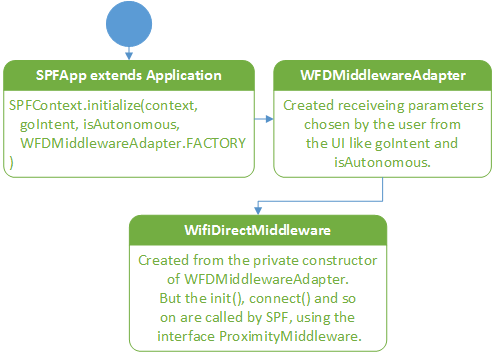
\includegraphics[scale=0.5]{./images/chap2/uml-parte0-1.png}
	\caption{General flow from SPFApp to the middleware}
	\label{uml-part0-1}
\end{figure}	

After that, as you can see in Figure \ref{uml-part0-1}, \textsf{WFDMiddlewareAdapter} (the most important class included into the \textsf{wpdadapter}'s package of the middleware) will be created and automatically it will instantiate the \textsf{WifiDirectMiddleware} object (the most important class included into the \textsf{wfd}'s package of the middleware). This process completes only with the creation of this last object, because the real initialization process and connection are made by SPF using the \textsf{ProximityMiddleware} interface. I'll discuss more in details these aspects during this document.
At the moment, i want to explain only the events used to send messages into the middleware. The main idea was to prevent most of the cyclic dependencies that Wi-Fi Direct APIs force to use. To do that, I used a library called \emph{Otto}. 
\emph{Otto} is an event bus designed to decouple different parts of your application while still allowing them to communicate efficiently. Forked from \emph{Guava}, \emph{Otto} adds unique functionality to an already refined event bus as well as specializing it to the Android platform.
To be able to post events in all Threads, I used a wrapper called \textsf{Ninebus}. But, the only difficulty to use \emph{Otto} is how maintain an ordered structure. 

\begin{figure}[thpb]
	\centering
	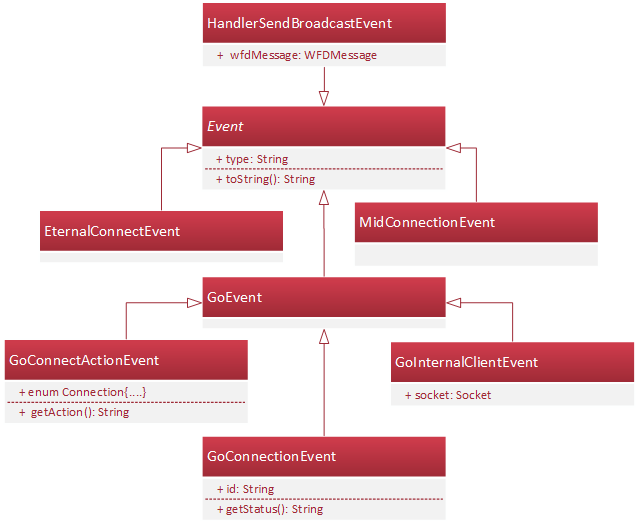
\includegraphics[scale=0.7]{./images/chap2/event-hyerarchy.png}
	\caption{Enter hierarchy}
	\label{event-hieranchy}
\end{figure}	

\begin{figure}[thpb]
	\centering
	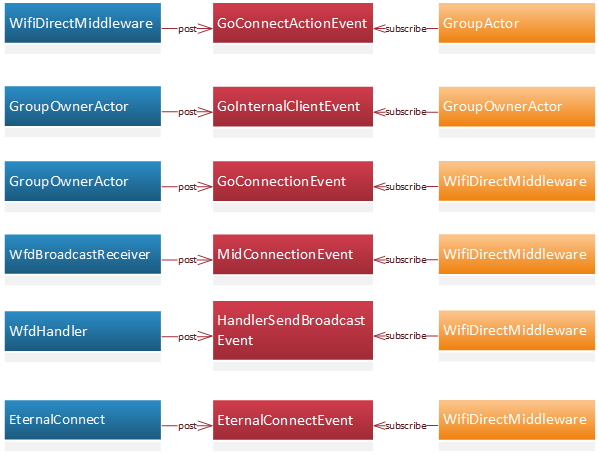
\includegraphics[scale=0.7]{./images/chap2/event-subscribe-post.png}
	\caption{Event post/subscribe responsibilities}
	\label{event-subscribe-post}
\end{figure}	

To achieve this, I used a package with all events inside, organized using the Java hierarchy. The complete class diagram of all events is in Figure \ref{event-hieranchy}.
Another important thing is to understand which class posts an event and which will reacts to it. To explain in a very simple way this fact, I created the diagram in Figure \ref{event-subscribe-post}. As you can see:
\begin{itemize}
	\item the blue elements are the classes the post events;
	\item in red there are all events;
	\item in orange are represented all subscribers.
\end{itemize}

This means, for example, that \textsf{WifiDirectMiddleware.java} posts a \textsf{GoConnectActionEvent} and \textsf{GroupActor} will catch the events and it will react to its, executing a method annotated with \textsf{@Subscribe}.

\section{Architecture}

\begin{figure}[thpb]
	\centering
	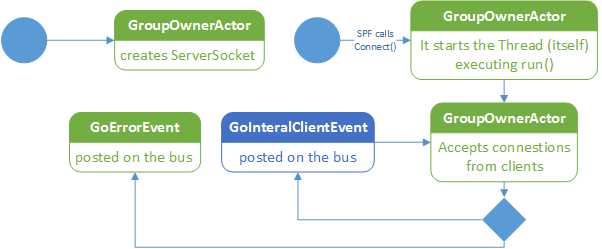
\includegraphics[scale=0.5]{./images/chap2/uml-parte0-2.png}
	\caption{GroupActor post behavior}
	\label{uml-part0-2}
\end{figure}	

\begin{figure}[thpb]
	\centering
	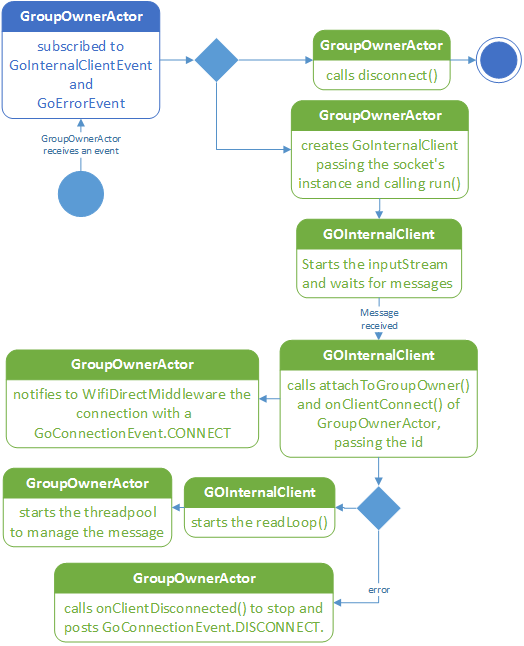
\includegraphics[scale=0.6]{./images/chap2/uml-parte0-3.png}
	\caption{GroupActor subscribe behavior}
	\label{uml-part0-3}
\end{figure}	

I don't want to explain in details the code of this middleware, instead, I want to show the structure and the interactions of the classes inside the wfd/groups package.
I created two different scheme to describe this. They are represented as state diagram because very simple to read, but probably the best type of UML could be the Sequence Diagram.
First, I want to describe how \textsf{GroupActor} and its subclasses post events. As you can see in Figure \ref{uml-part0-2}, when \textsf{GroupOwnerActor} starts, it will create a \textsf{ServerSocket}, nothing more. It's SPF that calling \textsf{connect()} will start the \textsf{GroupOwnerActor}'s thread executing its \textsf{run()} method. Inside of its, it will start to listen and accept clients connections. If everything will be ok, it will post a \textsf{GoInternalClientEvent} on the bus, otherwise a \textsf{GoErrorEvent}. In the first case, it will return to listen and accept other clients, forced by a while cycle. Obviously, this is only an extreme abstraction. To understand more in detail this, look the Figure \ref{uml-part0-3}, where I represented the sequence of operations when \textsf{GroupOwnerActor} receives the \textsf{GoInternalClientEvent} posted by itself (from its \textsf{run()} method and for this reason from another Thread).
When \textsf{GroupOwnerActor} receives this event, it will create and start a \textsf{GoInternalClient}, passing the socket instance. After that, this last thread starts the InputStream and waits for messages. 
When it receive a message, it calls \textsf{attachToGroupOwner()} and \textsf{onClientConnect()} of \textsf{GroupOwnerActor}, passing the identifier of the profile. These calls are necessary to notify to the \textsf{WifiDirectMiddlware} what happened, but the real logic will continue into the method \textsf{readLoop()} inside the \textsf{GoInternalClient} that starts the threadpool into \textsf{GroupOwnerActor} to manage the message. All these operations written here are perfectly represented in Figure \ref{uml-part0-3}.


\subsection{Class structure}

\begin{figure}[thpb]
	\centering
	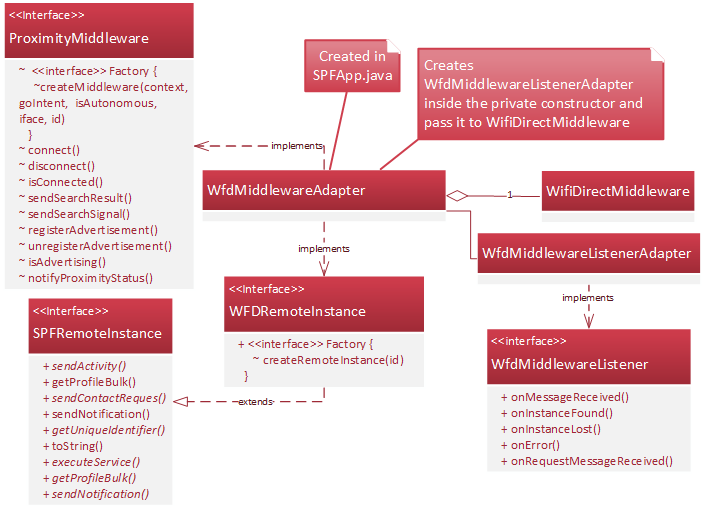
\includegraphics[scale=0.5]{./images/chap2/uml-parte1.png}
	\caption{Middleware's initial Class Diagram}
	\label{uml-part1}
\end{figure}	

\begin{figure}[thpb]
	\centering
	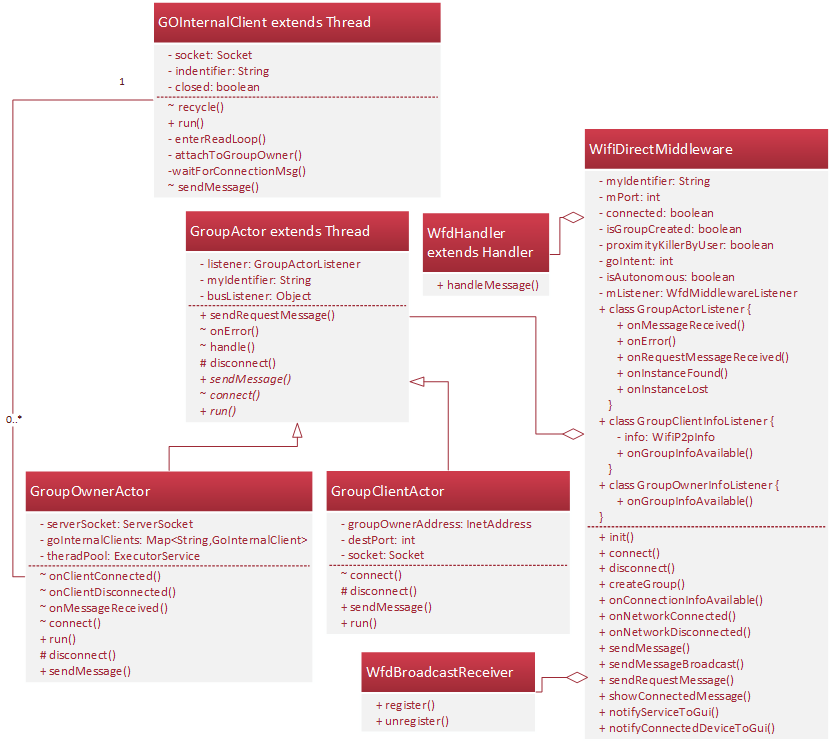
\includegraphics[scale=0.6]{./images/chap2/uml-parte2.png}
	\caption{Middleware's groups management Class Diagram}
	\label{uml-part2}
\end{figure}	


Now, I want to explain quickly the class structure of this middleware. Because there is a huge number of classes, I selected only a subset of these, as you can see in Figures \ref{uml-part1} and \ref{uml-part2}.
I cannot and I don't want to explain in details all classes and methods, because it's impossibile. Also, I don't want to repeat the same things for \textsf{GroupActor} and its subclasses. In this subsection, I want to explain some key feature of this new implementation of \textsf{WifiDirectMiddleware.java}.
In fact, there are some new important variable, like \textsf{isAutonomous} and \textsf{goIntent}. These variables are important, because chosen by the user from the UI. The first one is connected to the state of the switch ``Group Owner" and the second one to the switch ``Autonomous". 
I implemented a quick workaround to achieve this, by passing variables during the creation of the Middleware and updating these values after every change of switches. Obviously, this is not good and I'll explain why into Section \ref{conclusion}.


\section{Eternal Connect}

\emph{Eternal Connect} is a solution to restart discovery and connect phases after any network errors. This can be considered an improved version of the 	\emph{Eternal Discovery} that I used in \seqsplit{https://github.com/deib-polimi/PigeonMessanger}, because with this latest implementation, SPF will re-connect automatically trying every 15 second for 4 times. Obviously, you can configure this to achieve the best performances. Also, you can improve \emph{Eternal Connect} in different ways to obtain better performances during network's creation, in particular on the Group Owner in Autonomous mode. All the code related to \emph{Eternal Connect} is into a single class called \textsf{EternalConnect.java}.
\emph{Eternal Connect} has two different modes:
\begin{enumerate}
	\item standard: with automatic reconnection in a loop cycle for 4 times every 15 seconds.
	\item simple: with a single automatic reconnection. If it fails, it will stop.
\end{enumerate}
These two modes are partially implemented, because I created only the necessary features. If you need a different behavior, you can simply modify \textsf{onEternalConnectUpdate} that catches \textsf{EternalConnectEvent} in \textsf{WifiDirectMiddleware.java}. \textsf{EternalConnect.java} is a singleton class with these important public methods:
\begin{itemize}
	\item \textsf{eternalConnect()}: start the \emph{EternalConnect} as you can see in Listing 	\ref{eternalConnect}.
	\item \textsf{onNetworkDisconnected()}: if a device isn't a GO in Autonomous mode, this method will restart the \emph{Eternal Connect}, otherwise it will post an \textsf{EternalConnectEvent} to specify the ``simple reconnection" mode;
	\item \textsf{onConnectFailed()}: called when Wi-Fi Direct fails during the connection procedure, to restart the \emph{Eternal Connect} in standard mode;
	\item \textsf{onGroupCreationFailed()}: called when Wi-Fi Direct fails during the group creation procedure, to restart the \emph{Eternal Connect} in ``simple mode";
	\item \textsf{eternalCompletedSuccessfully()}: to complete the procedure, because the connection is established.
\end{itemize}


\begin{lstlisting}[caption={eternalConnect() method},label=eternalConnect, language=Java]
void eternalConnect(boolean proximityKilledByUser) {
  killScheduler();
  scheduler = Executors.newScheduledThreadPool(1);
    final Runnable runnable = new Runnable() {
      public void run() {
        if (proximityKilledByUser) {
        	  killScheduler();
          eternalCounter = 0;
          return;
        }	
		if (eternalCounter > MAX_ETERNAL_COUNT) {
          killScheduler();
          eternalCounter = 0;
        } else {
        	  //post EternalConnectEvent.NEW_EC_CYCLE
          eternalCounter++;
        }
	}
};

final ScheduledFuture<?> eternalHandle =
  scheduler.scheduleAtFixedRate(runnable, 
    10, 15, TimeUnit.SECONDS);
  scheduler.schedule(new Runnable() {
    public void run() {
      eternalHandle.cancel(true);
    }
  }, 15, TimeUnit.SECONDS);
}
\end{lstlisting}


\section{Wi-Fi Direct's known issues}

In this section i want to create a list with some of the known issues of Wi-Fi Direct protocol on Android devices.
\begin{itemize}
	\item There are random errors when you are trying to establish a connection. In most of the cases, to fix this problem you must kill the Wi-Fi Connection manually.
	\item The discovery procedure is absolutely unreliable. Sometime a device can't discover other devices without any reason and the only way to fix this problem is a stop, followed by a restart of the discovery procedure.
	\item Connection between different devices with different Android versions and manufacturers can be unstable.
	\item The most important problem in SPF2 is related to autonomous group \emph{join} operation. Because, if a device want to \emph{join} to a previously created group, it should ask to the GO the ``permission". In Android API there isn't a \textsf{join()} method (in \emph{wpa\_supplicant} yes, obviously), but there is the standard \textsf{connect()} method. This is not a big problem, instead the real problem is that if a device want to \emph{join}, on the GO will appear a popup. If the GO accepts the \emph{join} procedure, the connection can be completed. This process can't be automated and requires always the user's interaction. Also, for absolutely inexplicable reasons, when the connection with a third device starts, the entire group can be destroyed to try to recreate it quickly. This is a famous problem that you can found everywhere on \emph{stackoverflow}. At the moment there aren't any solutions. If you want to use \emph{wpa\_supplicant} from command line, this problem never happens, this implies that is caused by the Android implementation of Wi-Fi Direct. Also, the main consequence related to this problem is that sometime the group won't be recreated, caused by problems during connection or discovery phases. To be able to create a group of three devices with SPF2, you should try many times to obtain the desired result. This is a huge Android's implementation issue, impossibile to fix, at the moment.
\end{itemize}


